% Autor: Simon May
% Datum: 2017-10-05
% Diese Datei bietet ein minimalistisches Grundgerüst für ein LaTeX-Dokument,
% z.B. für die Bearbeitung der Aufgaben.
\documentclass[
	% Papierformat
	a4paper,
	% Schriftgröße (beliebige Größen mit „fontsize=Xpt“)
	12pt,
	% Schreibt die Papiergröße korrekt ins Ausgabedokument
	pagesize,
	% Sprache für z.B. Babel
	ngerman
]{scrartcl}

% Achtung: Die Reihenfolge der Pakete kann (leider) wichtig sein!
% Insbesondere sollten (so wie hier) babel, fontenc und inputenc (in dieser
% Reihenfolge) als Erstes und hyperref und cleveref (Reihenfolge auch hier
% beachten) als Letztes geladen werden!

% Silbentrennung etc.; Sprache wird durch Option bei \documentclass festgelegt
\usepackage{babel}
% Verwendung der Zeichentabelle T1 (Sonderzeichen etc.)
\usepackage[T1]{fontenc}
% Legt die Zeichenkodierung der Eingabedatei fest, z.B. UTF-8
\usepackage[utf8]{inputenc}
% Schriftart
\usepackage{lmodern}
% Zusätzliche Sonderzeichen
\usepackage{textcomp}

% Mathepaket (intlimits: Grenzen über/unter Integralzeichen)
\usepackage[intlimits]{amsmath}
% Ermöglicht die Nutzung von \SI{Zahl}{Einheit} u.a.
\usepackage{siunitx}
% Zum flexiblen Einbinden von Grafiken (\includegraphics)
\usepackage{graphicx}
% Abbildungen im Fließtext
\usepackage{wrapfig}
% Abbildungen nebeneinander (subfigure, subtable)
\usepackage{subcaption}
% Funktionen für Anführungszeichen
\usepackage{csquotes}
% Zitieren, Bibliographie
\usepackage{biblatex}

% Verlinkt Textstellen im PDF-Dokument
\usepackage[unicode]{hyperref}
% "Schlaue" Referenzen (nach hyperref laden!)
\usepackage{cleveref}

% siunitx: Deutsche Ausgabe, Messfehler getrennt mit ± ausgeben
\sisetup{
	locale=DE,
	separate-uncertainty
}

\begin{document}
\begin{titlepage}
	\centering
	{\scshape\LARGE Versuchsbericht zu \par}
	\vspace{1cm}
	{\scshape\huge Raster-Tunnel-Mikroskopie, Spitzenpräparation und Messungen an Graphit und Gold     \par}
	\vspace{2.5cm}
	{\LARGE Gruppe 6 Mo\par}
	\vspace{0.5cm}
	{\large Nils Kulawiak (E-Mail: n\_kula01@wwu.de) \par}
	{\large Oliver Brune (E-Mail: o\_brun02@wwu.de) \par}
	{\large Anthony Pietz (E-Mail: a\_piet09@wwu.de) \par}
	\vfill
	durchgeführt am 17.12.2018\par
	
	\vfill
	betreut von Alexander Timmer\par
	
	\vfill
	{\large \today\par}
\end{titlepage}

\tableofcontents
		
\newpage
\section{Ergebnis}
Zuerst wird versucht die Pulsenergie des Lasers zu bestimmen. Dazu muss zuerst die niedrigste Spannung ermittelt werden. Das geschieht über

\begin{figure}[h!]
	\centering
	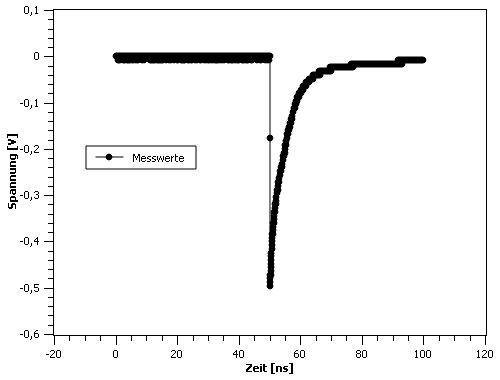
\includegraphics[scale=0.7]{Energie.png}
	\caption{}
	\label{Energie}
\end{figure}


Die geschieht über die Formel
\begin{equation}
E_{p} = \dfrac{1 \mu J}{50mV}U_{min} = \SI{9,92 \pm 0,30}{J}.
\end{equation}



\newpage
\begin{thebibliography}{9}
	\bibitem{A}
	J. Bardeen, Phys. Rev. Lett. 6, 57 (1961).
	
	\bibitem{B}
	J. Tersoff, D. R. Hamann, Phys. Rev. Lett. 50, 1998 (1983)
	
	\bibitem{C}
	\textit{Raster-Tunnel-Mikroskop, Spitzenpräparation und Messungen an Graphit und Gold },
	FD-Praktikum, (2010)

\end{thebibliography}
\end{document}